\subsubsection{Scope}

\begin{figure}[H]
	\centering
	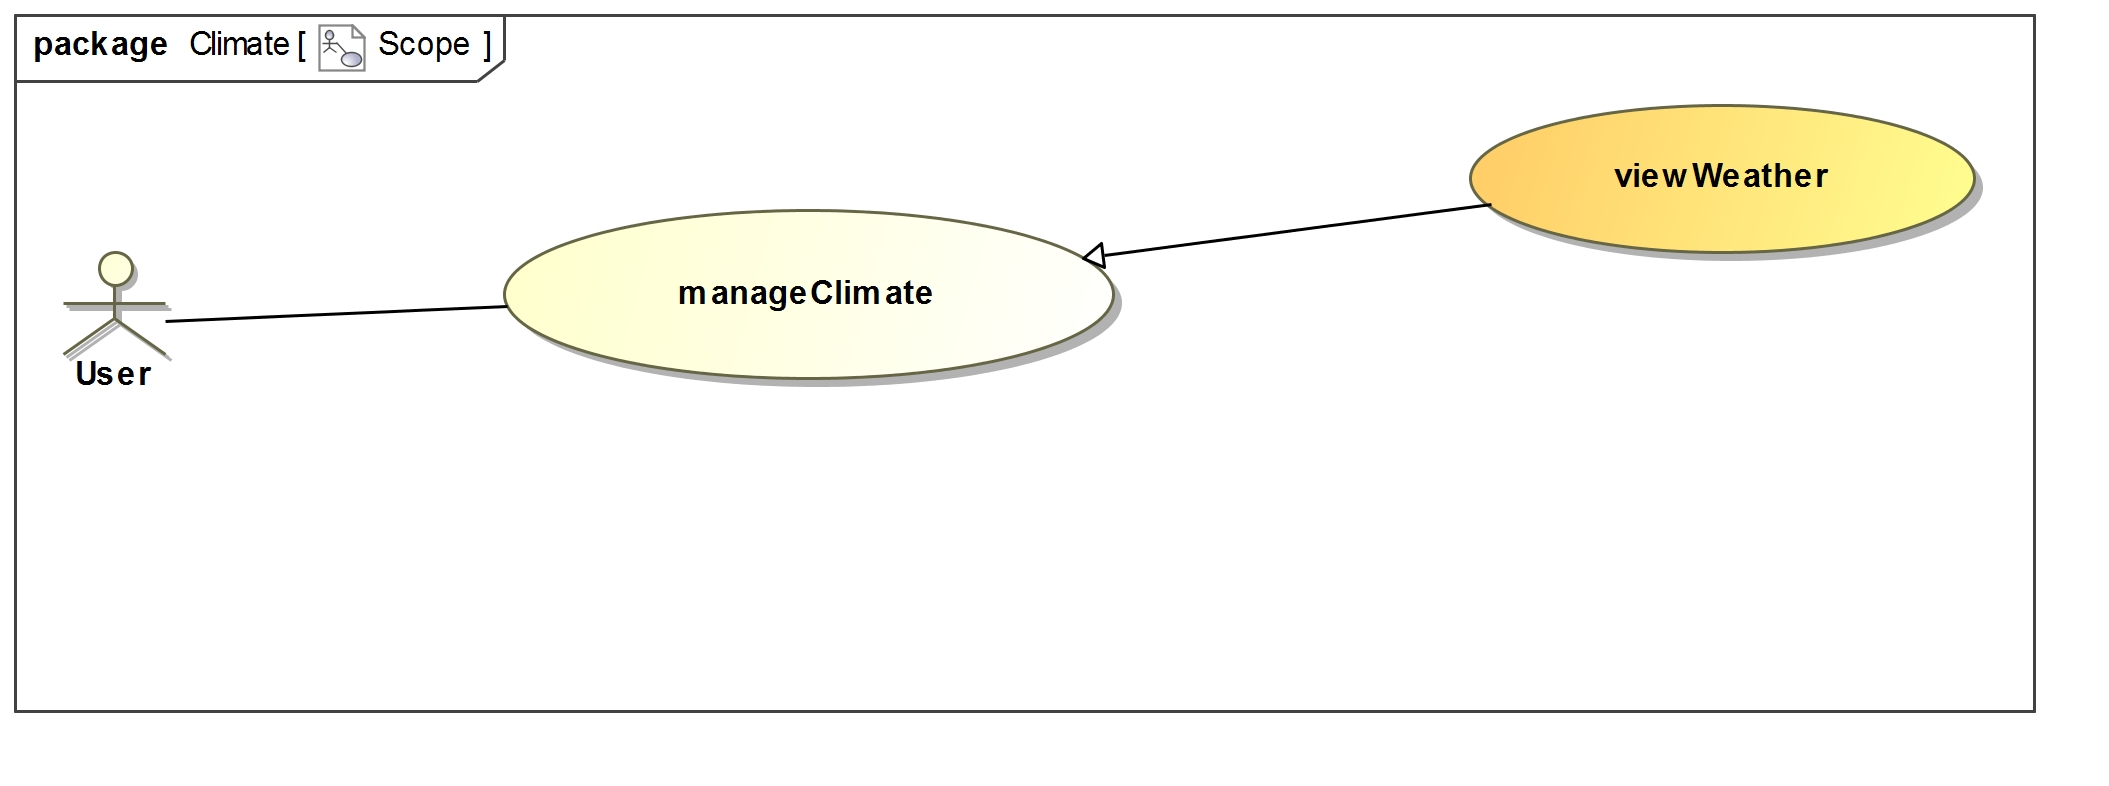
\includegraphics[scale=0.3]{../images/funcReq/ClimateScope.jpg}
	\caption{The scope of functionality required from the climate module \label{overflow}}
\end{figure} Users are able to view weather and query forecasts.

\subsubsection{viewWeather}

A user can view weather by going on to the weather tab on the system. The user is able to see weather for a specific place by specifying the name of that place in a search bar. Below are the service contract, activity diagram and functional requirements diagram for viewWeather.

\begin{figure}[H]
	\centering
	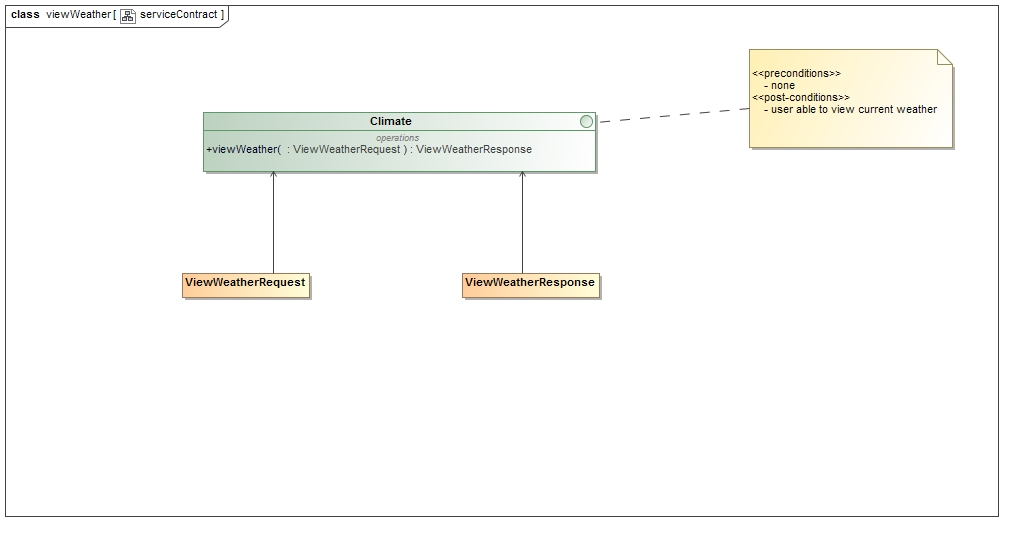
\includegraphics[scale=0.23]{../images/funcReq/viewWeatherServiceContract.jpg}
	\caption{The service contract for viewWeather \label{overflow}}
\end{figure}

\begin{figure}[H]
	\centering
	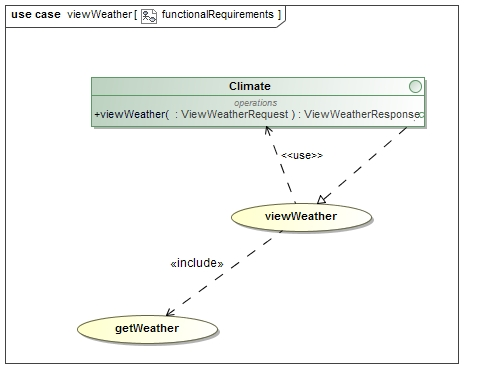
\includegraphics[width=1.0\textwidth]{../images/funcReq/viewWeatherFunctionalRequirements.jpg}
	\caption{The functional requirements diagram for viewWeather \label{overflow}}
\end{figure}

\begin{figure}[H]
	\centering
	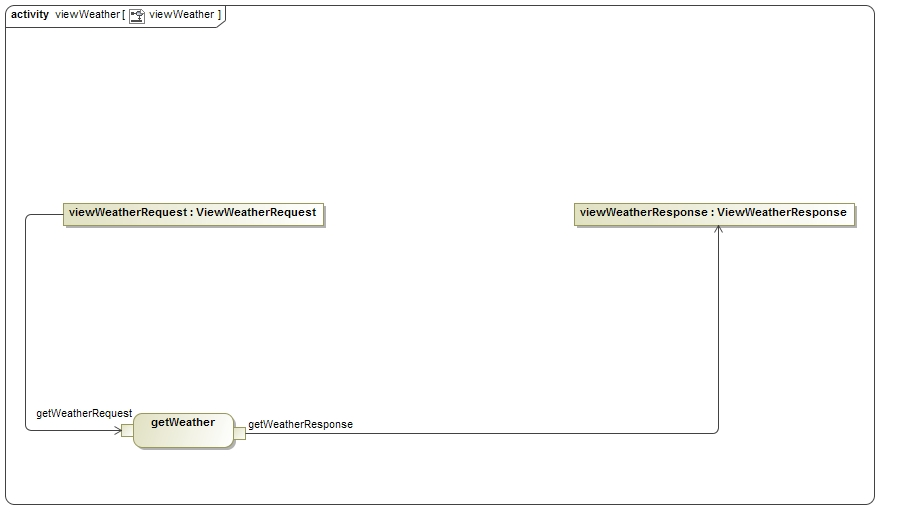
\includegraphics[scale=0.2]{../images/funcReq/viewWeatherActivityDiagram.jpg}
	\caption{The activity diagram for viewWeather \label{overflow}}
\end{figure}